\documentclass[a4paper]{article}

\usepackage[T1]{fontenc}
\usepackage[english]{babel}

\usepackage{hyperref}
\hypersetup{%
    pdfauthor = {Tobias Andersson, Victor Koronen},
    pdftitle = {ID1217: The Green Elevator},
    pdfsubject = {ID1217},
    pdfkeywords = {parallel programming},
    pdfcreator = {LaTeX with hyperref package},
    pdfproducer = {pdflatex}
}

\usepackage{graphicx}

\title{ID1217: ``The Green Elevator''}
\author{%
    Tobias Andersson <\href{mailto:tobias2@kth.se}{tobias2@kth.se}> \and
    Victor Koronen <\href{mailto:koronen@kth.se}{koronen@kth.se}>
}
\date{\today}

\begin{document}

\maketitle
\thispagestyle{empty}

\section{Introduction}

Our task was to design, implement and evaluate a controller for a simulated set
of elevators, see finure \ref{fig:hardware_control_panel}.

\begin{figure}[p]
    \centering
    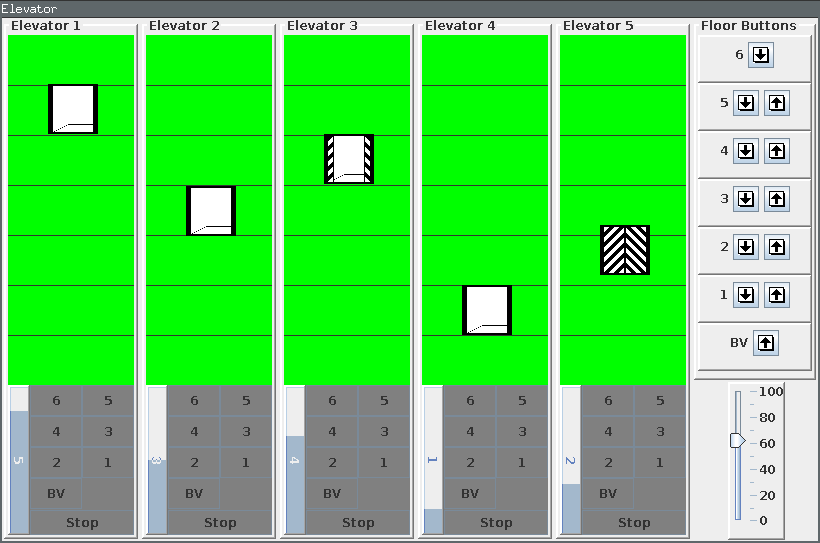
\includegraphics[width=1.0\textwidth]{images/elevators_5_6.png}
    \caption{The hardware control panel.}
    \label{fig:hardware_control_panel}
\end{figure}

\section{Implementation}

We decided to implement the controller application in Java, since it is a
language we both felt comfortable with. This also allowed us to utilize classes
from the extensive Java Standard Library and to develop the program using the
Eclipse IDE. We mainly developed the controller application in our laptops,
which both run a recent edition of the GNU/Linux Ubuntu OS.

The controller application consists of a set of classes with different
responsibilities.

% Describe your implementation (functions, classes, interfaces).
\begin{description}

\item[\texttt{se.kth.id1217.Main}] The main entry point to the controller
    program. Parses command line parameters, sets up the network connection and
    passes control over to \texttt{se.kth.id1217.MasterController}.

\item[\texttt{se.kth.id1217.MasterController}] Receives messages from the
    hardware. Decides which elevator should respond to floor button presses and
    passes cabin button presses onto an instance of
    \texttt{se.kth.id1217.ElevatorController}.

\item[\texttt{se.kth.id1217.ElevatorController}] The control unit for one of the
    elevators. Each elevator has a separate instance of this class. Manages the
    route for this elevator and controlls the motors.

\end{description}

\section{Algorithms}
% Describe algorithms you have developed (chosen), synchronization or/and
% communication mechanisms you have used, and explain motivation for your design
% choices.

\section{Evaluation}
% Present and explain your performance evaluation results, if any.

\section{Summary and conclusions}
% Give a summary of your achievements. In particular, explain briefly what you
% learned from the assignment and any problems you may have encountered. You
% are also welcome to suggest changes to the assignment in order to improve it.

\end{document}
